\documentclass{beamer}
%\usepackage{xspace}
\usepackage{amsmath,amssymb}
\usepackage{graphicx}
%\usepackage{svg}
%\usepackage{pgfpages}
%\pgfpagesuselayout{4 on 1}[a4paper,border shrink=5mm,landscape]
%\usepackage{psfrag}
%\usepackage[usenames,dvipsnames]{xcolor}
\usepackage{braket}
\usepackage{tikz}
\usetikzlibrary{graphs}
\usetikzlibrary{datavisualization}
\usetikzlibrary{datavisualization.formats.functions}
\usepackage{pgfplotstable}
\usepgfplotslibrary{patchplots}

\setbeamercovered{transparent}

\usetheme{Pittsburgh}
%\usetheme{default}

\setbeamertemplate{sidebar right}{}
\setbeamertemplate{footline}[frame number]
%\usefonttheme{professionalfonts}

%\usepackage{sansmathaccent}
%\usepackage{bm}

%\usepackage{unicode-math}
%%\setmainfont[SlantedFont={Latin Modern Roman Slanted},SlantedFeatures={Color=000000},
%%  SmallCapsFont={TeX Gyre Termes},SmallCapsFeatures={Letters=SmallCaps}]{XITS}
%\setmathfont[math-style=ISO,sans-style=upright]{XITS Math}
%\setmathfont[range={\mathcal,\mathbfcal}]{Latin Modern Math}

\usepackage{sfmath}

%\mathversion{sans}

\newcommand{\Tr}{\mathsf{Tr}}

\definecolor{redorange}{rgb}{1.0, .25, .25}
\definecolor{citation}{rgb}{.1, 0.8, .35}
\newcommand\emm[1]{\textcolor{redorange}{{#1}}}
\newcommand\numc[1]{\textcolor{citation}{{\bf #1}}}

%\newcommand\bm[1]{{\mbox{\boldmath $#1$}}}
\newcommand\bm[1]{{\mathbf{#1}}}
%\newcommand\bm[1]{{\bf #1}}
%\newcommand\bm[1]{\ensuremath{\boldsymbol{#1}}}
%\newcommand\bm[1]{{\textbf{\it #1}}}

\title{Nonlocality}
\author{Ryuhei Mori}
%\institute{$\vcenter{\hbox{\includegraphics[width=30pt]{ELC_logo}}}$ Postdoctoral Fellow of ELC\\ $\vcenter{\hbox{\includegraphics[width=20pt]{titech_logo}}}$ Tokyo Institute of Technology}
\institute{Tokyo Institute of Technology}
%\date{21, Feb, 2019}



\begin{document}
\begin{frame}[plain]
\maketitle
\end{frame}



\begin{frame}{Bell test: CHSH game (1964, 1969)}
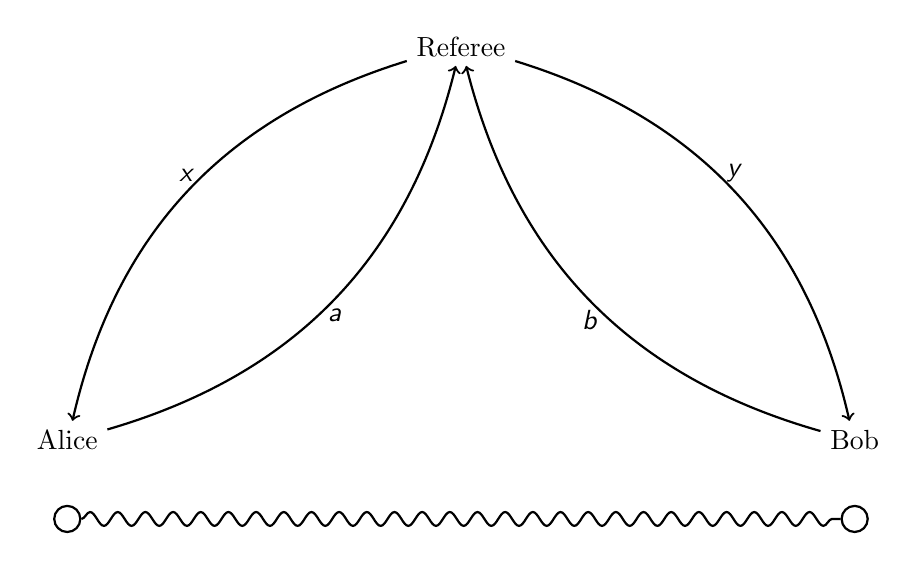
\begin{tikzpicture}
\node at (5,5) (R) {Referee};
\node at (0,0) (A) {Alice};
\node at (10,0) (B) {Bob};
\node at (0,-1)[circle,thick,draw] (As) {};
\node at (10,-1)[circle,thick,draw] (Bs) {};
\draw[->,thick] (R) edge[bend right] node[anchor=south, midway]{$x$} (A);
\draw[->,thick] (R) edge[bend left] node[anchor=south, midway]{$y$} (B);
\draw[->,thick] (A) edge[bend right] node[anchor=north, midway]{$a$} (R);
\draw[->,thick] (B) edge[bend left] node[anchor=north, midway]{$b$} (R);
\draw[thick,decorate,decoration=snake] (As) -- (Bs);
\end{tikzpicture}
%\includegraphics[width=30pt]{Alice_in_Wonderland.png}
\begin{center}
Alice and Bob win iff $\emm{a\oplus b = x\wedge y}$.
\end{center}
\end{frame}

\begin{frame}{Bell inequality}
$a_x$: Output of Alice for given $x$.

$b_y$: Output of Bbob for given $y$.
\begin{align*}
a_0 \oplus b_0 &= 0\\
a_1 \oplus b_0 &= 0\\
a_0 \oplus b_1 &= 0\\
a_1 \oplus b_1 &= 1
\end{align*}
By adding all equations, we get $0=1$, which means there is no solution.
Hence, the winning probability 1 cannot be achieved.

\vspace{1em}
Three equalities can be satisfied, so that the largest winning probability is \emm{3/4}~(Bell inequality or CHSH inequality).

\vspace{1em}
If Alice and Bob share quantum states, then the largest winning probability is
$(2+\sqrt{2})/4\approx \emm{0.854}$~(Violation of Bell/CHSH inequality)
\end{frame}

\begin{frame}{Locality (Hidden variable model)}
\begin{center}
Joint preparation and independent measurements.
\end{center}
Probability distribution $P(a,b\mid x,y)$ is said to be \emm{local} if
\begin{equation*}
P(a, b\mid x,y) = \sum_{\lambda} P(\lambda) P(a\mid x, \lambda) P(b\mid y,\lambda).
\end{equation*}
\vspace{2em}
\begin{center}
Quantum physics allow \emm{nonlocal} behaviors.
\end{center}
\end{frame}

\begin{frame}{Joint probability distribuion}
\small
\begin{lemma}
\begin{equation*}
P(a, b\mid x,y) = \sum_{\lambda} P(\lambda) P(a\mid x, \lambda) P(b\mid y,\lambda).
\end{equation*}
if and only if
\begin{equation*}
P(a, b\mid x,y) = \sum_{a_x = a,\, b_y = b} q(a_0, a_1, b_0, b_1).
\end{equation*}
\end{lemma}
\begin{proof}
$(\Rightarrow)$
\begin{align*}
q(a_0,a_1,b_0,b_1) &:= \sum_{\lambda}P(\lambda) P(a_0\mid x=0, \lambda) P(a_1\mid x=1, \lambda)\\
&\cdot P(b_0\mid y=0, \lambda) P(b_1\mid y=1, \lambda)
\end{align*}
$(\Leftarrow)$
\end{proof}
\end{frame}

\begin{frame}{Einstein--Podolsky--Rosen (EPR) paradox (1935)}
\begin{equation*}
P(a, b\mid x,y) = \sum_{\lambda} P(\lambda) P(a\mid x, \lambda) P(b\mid y,\lambda).
\end{equation*}
$\iff$
there exists a joint distribution of $(a_0,a_1,b_0,b_1)$.

\begin{center}
\Large
$\Downarrow$

\vspace{1.0em}
\normalsize
In quantum physics,
$a_0,a_1,b_0,b_1$ \emm{cannot \textit{exists}} simultaneously.

\vspace{1.0em}
\Large
$\Downarrow$

\vspace{1.0em}
\normalsize
In quantum physics,
position and momentum \emm{cannot \textit{exists}} simultaneously.
\end{center}

%[Einstein, Podolsky, Rosen 1935, \numc{15771}]
\end{frame}




\end{document}
